% Chapter Template

\chapter{Results} % Main chapter title

\label{Chapter 3} % Change X to a consecutive number; for referencing this chapter elsewhere, use \ref{ChapterX}





%
%\rowcolors{2}{gray!6}{white}
%
%\begin{table}
%%	\captionsetup{font=small}
%	\caption{\label{tab:MLCA-level1}Level 1 classes comparison in the first step of MLCA. (All data, n = 6155, 24483 data points)}\vspace{-0.3cm}
%	\centering
%	\fontsize{9}{10}\selectfont
%	\begin{tabular}[t]{cccccccc}
%		\hiderowcolors
%		\toprule
%		\Centerstack{N of \\ classes} & \Centerstack{N of free \\ parameters} & log-likelihood & AIC & BIC & aBIC & Entropy & \Centerstack{ Lo-Mendel-Rubin \\ LRT}   \\
%		\midrule
%		\showrowcolors
%		1 & 48 & -372017.3 & 744130.6 & 744519.7 & 744367.1 & -- & --\\
%		2 & 97 & -368913.7 & 738021.4 & 738807.7 & 738499.4 & 0.777 & < 0.0001\\
%		3 & 146 & -366665.0 & 733621.9 & 734805.4 & 734341.4 & 0.666 & < 0.0001\\
%		4 & 195 & -365528.6 & 731447.1 & 733027.7 & 732408.0 & 0.658 & 0.8478\\
%		5 & 244 & -364901.2 & 730290.3 & 732268.1 & 731492.7 & 0.648 & 0.7602\\
%		6 & 293 & -363641.8 & 727869.5 & 730244.5 & 729313.4 & 0.701 & 0.7632\\
%		7 & 342 & -362789.9 & 726263.7 & 729035.9 & 727949.0 & 0.729 & 0.7702\\
%		8 & 391 & -362047.9 & 724877.9 & 728047.2 & 726804.6 & 0.737 & 0.8261\\
%		\bottomrule
%		\multicolumn{8}{l}{\textit{Note: }}\\
%		\multicolumn{8}{l}{\textbf{Abbreviations:} MLCA, multilevel class analysis; N, number; AIC, Akaike information criterion; BIC, }\\
%		\multicolumn{8}{l}{Bayesian information criterion; aBIC, adjusted BIC; Entropy, a pseudo-r-squared index; Lo-Mendel-Rubin}\\
%		\multicolumn{8}{l}{LRT, likelihood ratio test comparing $q$ classes models with $q-1$ classes models.}\\
%	\end{tabular}
%\end{table}
%
%\rowcolors{2}{white}{white}


\begin{figure}
	%\vspace*{13cm}
	\centering
	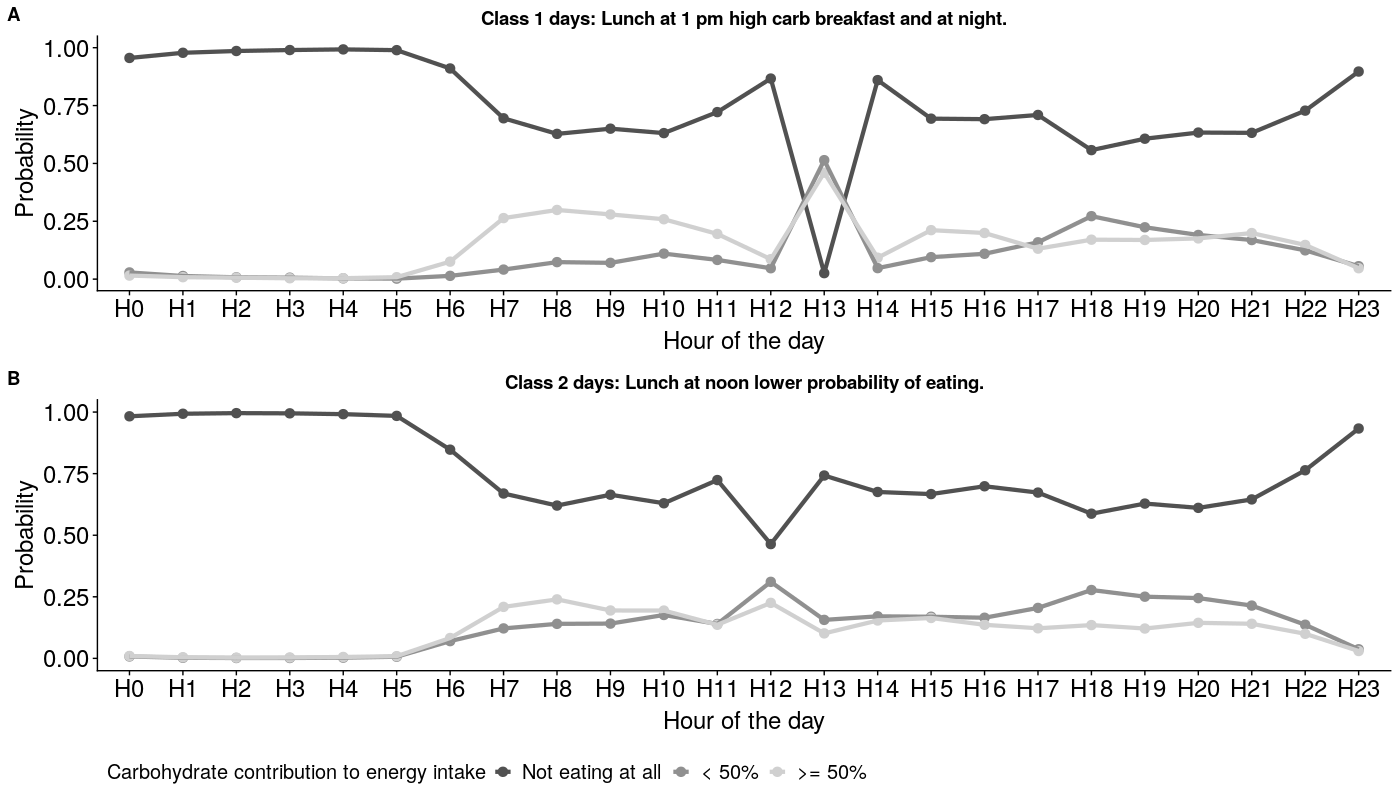
\includegraphics{Figures/class1mlcalevel1.png}
	\decoRule
	\caption[Level 1 Classes in MLCA]{Carbohydrate temporal eating patterns at observational day level.}
	\label{fig:MLCAfig1}
\end{figure}
%%\end{verbatim}



\rowcolors{2}{gray!6}{white}
\begin{table}
	
	\caption{\label{tab:}Fit Criteria for Each Model Specification}
	\centering
	\fontsize{9}{11}\selectfont
	\begin{tabular}[t]{lccccc}
		\hiderowcolors
		\toprule
		\multicolumn{1}{c}{ } & \multicolumn{5}{c}{Number of level 1 classes} \\
		\cmidrule(l{2pt}r{2pt}){2-6}
		Model & 1 class & 2 classes & 3 classes & 4 classes & 5 classes\\
		\midrule
		\showrowcolors
		\addlinespace[0.3em]
		\multicolumn{6}{l}{\textbf{Fixed effects model}}\\
		\hspace{1em}No. of free parameters & 48 & 97 & 146 & 195 & 244\\
		\hspace{1em}\hspace{1em}Log-likelihood & -372017.293 & -368913.708 & -366664.971 & -365528.553 & -364901.166\\
		\hspace{1em}\hspace{1em}BIC & 744519.661 & 738807.672 & 734805.379 & 733027.723 & 732268.13\\
		\hspace{1em}\hspace{1em}Lo-Mendell-Rubun LRT & --- & < 0.0001 & < 0.0001 & 0.8478 & 0.7602\\
		\hspace{1em}\hspace{1em}Entropy & 1 & 0.777 & 0.666 & 0.658 & 0.648\\
		\addlinespace[0.3em]
		\multicolumn{6}{l}{\textbf{Random effects model}}\\
		\hspace{1em}2 between classes &  &  &  &  & \\
		\hspace{1em}\hspace{1em}No. of free parameters &  & 195 & 293 & 391 & \\
		\hspace{1em}\hspace{1em}Log-likelihood &  & -363460.153 & -361571.164 & -360297.394 & \\
		\hspace{1em}\hspace{1em}BIC &  & 728890.925 & 726103.308 & 724546.13 & \\
		\hspace{1em}\hspace{1em}Entropy &  & 0.834 & 0.798 & 0.784 & \\
		\hspace{1em}3 between classes &  &  &  &  & \\
		\hspace{1em}\hspace{1em}No. of free parameters &  & 293 & 440 & 587 & \\
		\hspace{1em}\hspace{1em}Log-likelihood &  & -360910.13 & -358902.821 & -357404.521 & \\
		\hspace{1em}\hspace{1em}BIC &  & 724781.241 & 722252.166 & 720741.109 & \\
		\hspace{1em}\hspace{1em}Entropy &  & 0.824 & 0.793 & 0.824 & \\
		\hspace{1em}4 between classes &  &  &  &  & \\
		\hspace{1em}\hspace{1em}No. of free parameters &  & 391 & 587 & 783 & \\
		\hspace{1em}\hspace{1em}Log-likelihood &  & -358684.859 & -356668.354 & -355235.955 & \\
		\hspace{1em}\hspace{1em}BIC &  & 720078.473 & 719268.774 & 718384.699 & \\
		\hspace{1em}\hspace{1em}Entropy &  & 0.816 & 0.817 & 0.806 & \\
		\bottomrule
		\multicolumn{6}{l}{\textit{Note: }}\\
		\multicolumn{6}{l}{Abbreviation: No, number; BIC, Bayesian information criterion; Entropy, a pseudo-r-squared index;}\\ 
		\multicolumn{6}{l}{Lo-Mendel-Rubin LRT, likelihood ratio test comparing $q$ classes models with $q-1$ classes models.}\\
	\end{tabular}
\end{table}
\rowcolors{2}{white}{white}






%----------------------------------------------------------------------------------------
%	SECTION 1
%----------------------------------------------------------------------------------------

\section{Main Section 1}


\begin{table}[h]
	\rowcolors{2}{gray!6}{white}	
	\caption{\label{tab:MLCAtab1}Means, percentages, and 95\% CIs of the characteristics  of carbohydrate temporal eating patterns by MLCA memberships in the UK adults (NDNS RP 2008/09-2015/16, sample size = 6155).}\vspace{-0.3cm}
		\centering
		\fontsize{9}{10}\selectfont
		\begin{tabular}[t]{lccc}
			\hiderowcolors
			\toprule
			 & Latent class = 1 & Latent class = 2 & P value \textsuperscript{*}\\
			\midrule
			\showrowcolors
			Total (\%) & 66.4  (64.8 , 68.1) & 33.6  (31.9 , 35.2) & \\
			Countries (\%) &  &  & \\
			\hspace{1em}England & 83.1  (80.9 , 85.1) & 85.4  (83.0 , 87.5) & 0.203\\
			\hspace{1em}Northern Ireland & 3.0  (2.3 , 3.9) & 2.3  (1.7 , 3.1) & \\
			\hspace{1em}Scotland & 8.9  (7.2 , 11.0) & 7.7  (5.9 , 9.9) & \\
			\hspace{1em}Wales & 5.0  (4.1 , 6.0) & 4.6  (3.6 , 6.0) & \\
			Age (years) & 47.3 (46.4, 48.2) & 50.1 (49.1, 51.1) & < 0.001\\
			Sex (\%) &  &  & \\
			\hspace{1em}Men & 47.3  (45.2 , 49.5) & 51.0  (48.1 , 53.9) & 0.048\\
			\hspace{1em}Women & 52.7  (50.5 , 54.8) & 49.0  (46.1 , 51.9) & \\
			Survey years (\%) &  &  & \\
			\hspace{1em}1 & 13.1 (10.8, 15.8) & 15.0 (12.1, 18.5) & 0.365\\
			\hspace{1em}2 & 12.3 (10.1, 14.9) & 11.9 (9.4, 14.2) & \\
			\hspace{1em}3 & 12.0 (9.8, 14.8) & 10.4 (8.2, 13.1) & \\
			\hspace{1em}4 & 13.2 (10.9, 16.0) & 11.4 (9.0, 14.2) & \\
			\hspace{1em}5 & 13.0 (10.8, 15.7) & 13.9 (11.1, 17.3) & \\
			\hspace{1em}6 & 12.0 (9.9, 14.4) & 11.1 (8.8, 13.9) & \\
			\hspace{1em}7 & 12.3 (10.1,14.9) & 13.5 (10.9, 16.7) & \\
			\hspace{1em}8 & 12.0 (9.9, 14.5) & 12.8 (10.3, 15.8) & \\
			BMI (kg/m\textsuperscript{2}) & 27.2 (26.9, 27.5) & 27.7 (27.5, 28.1) & 0.007\\
			WC (cm) & 92.6 (91.9, 93.3) & 94.2 (93.1, 95.2) & 0.013\\
			Smoking status (\%) &  &  & \\
			\hspace{1em}Current & 19.8  (18.2 , 21.4) & 23.8 (21.3 , 26.5) & < 0.001\\
			\hspace{1em}Ex-smoker & 22.5  (20.8 , 24.2) & 28.0 (25.4 , 30.7) & \\
			\hspace{1em}Never & 57.8  (55.7 , 59.8) & 48.2 (45.3 , 51.1) & \\
			Current drinking status (\%) &  &  & \\
			\hspace{1em}Yes & 23.1  (21.3 , 25.1) & 11.1  (9.5 , 13.0) & < 0.001\\
			Hypertension (\%) \textsuperscript{\dag} &  &  & \\
			\hspace{1em}Yes & 27.4  (25.0 , 29.9) & 32.6  (29.3 , 36.1) & 0.012\\
			Total energy intake (KJ) & 7425.7 (7323.7, 7527.8) & 8149.9 (7997.3, 8302.7) & < 0.001\\
			Carbohydrate intake (g) & 226.0 (222.8, 229.3) & 210 (206.1, 213.9) & < 0.001\\
			Carbohydrate
			percent (\%) \textsuperscript{\ddag} & 48.3 (48.0, 48.6) & 40.9 (40.6, 41.3) & < 0.001\\
			Glucose (mmol/l) & 5.13 (5.09, 5.17) & 5.17 (5.11, 5.22) & 0.292\\
			A1C (\%) & 5.49 (5.47, 5.52) & 5.47 (5.44,5.51) & 0.264\\
			DM \textsuperscript{\S} & 4.1  (3.1 , 5.3 ) & 5.9  (4.3 , 8.0 ) & 0.061\\
			Physical
			activity (hours/day) \textsuperscript{\P} & 1.51 (1.39, 1.63) & 1.64 (1.45, 1.82) & 0.244\\
			\bottomrule
			\multicolumn{4}{l}{\textit{Note: }}\\
			\multicolumn{4}{l}{\textbf{Abbreviations}: CI, confidence intervals; MLCA, multilevel latent class analysis; NDNS RP, national}\\ 
			\multicolumn{4}{l}{dietary and nutrition survey rolling programme; BMI body mass index; WC, waist circumference; }\\
			\multicolumn{4}{l}{A1C, haemoglobin A1c;DM, diabetes mellitus; h, hour.}\\
			\multicolumn{4}{l}{Variables from the blood tests (glucose and A1C) are weighted by blood sample weights,}\\
			\multicolumn{4}{l}{the others are weighted by individual weights.}\\
			\multicolumn{4}{l}{Glucose and A1C levels are estimated in subgroups of people without diabetes.}\\
			\multicolumn{4}{l}{Variables from the blood tests (glucose and A1C) are weighted by blood sample weights,}\\  
			\multicolumn{4}{l}{the others are weighted by individual weights.}\\
			\multicolumn{4}{l}{Glucose and A1C levels are estimated in subgroups of people without diabetes.}\\
			\multicolumn{4}{l}{\textsuperscript{*} For continuous variables, the F test was used to determine differences between latent classes.}\\
			\multicolumn{4}{l}{For categorical variables, differences between latent classes were assessed using the adjusted}\\
			\multicolumn{4}{l}{Pearson Chi-2 test for survey data.}\\
			\multicolumn{4}{l}{\textsuperscript{\dag} Hypertension was defined as either systolic blood pressure >= 140 mmHg or diastolic blood}\\
			\multicolumn{4}{l}{pressure >= 90 mmHg, or under treatment for hypertension.}\\
			\multicolumn{4}{l}{\textsuperscript{\ddag} Carbohydrate percent indicates the percentage of energy from carbohydrate in total energy intake}\\
			\multicolumn{4}{l}{\textsuperscript{\S} DM was defined by A1C > 6.5\%.}\\
			\multicolumn{4}{l}{\textsuperscript{\P} Physical activity was calculated as mean time spent at moderate or vigorous physical activity}\\
			\multicolumn{4}{l}{during the survey.}\\
		\end{tabular}
	\rowcolors{2}{white}{white}
	\end{table}











%-----------------------------------
%	SUBSECTION 1
%-----------------------------------
\subsection{Subsection 1}


%-----------------------------------
%	SUBSECTION 2
%-----------------------------------

\subsection{Subsection 2}

%----------------------------------------------------------------------------------------
%	SECTION 2
%----------------------------------------------------------------------------------------

\section{Main Section 2}



\rowcolors{2}{gray!6}{white}

\begin{table}
	
	\caption{\label{tab:LCGAtab1}Means, percentages, and 95\% CIs of the characteristics of carbohydrate temporal eating patterns by LCGA memberships in the UK adults (NDNS RP 2008/09-2015/16, sample size = 6155).}\vspace{-0.3cm}
	\centering
	\fontsize{9}{11}\selectfont
	\begin{tabular}[t]{lcccc}
		\hiderowcolors
		\toprule
		 & Latent class = 1 & Latent class = 2 & Latent class = 3 & P value \textsuperscript{*}\\
		\midrule
		\showrowcolors
		Total (\%) & 28.4 (26.8, 30.1) & 7.0 (6.2, 7.9) & 64.6 (62.9, 66.2) & \\
		Countries (\%) &  &  &  & \\
		\hspace{1em}England & 81.4 (78.5, 84.0) & 87.5 (82.9, 91.0) & 84.6 (82.5, 86.4) & 0.004\\
		\hspace{1em}Northern Ireland & 3.9 (2.9, 5.1) & 0.6 (0.3, 1.2) & 2.5 (2.0, 3.2) & \\
		\hspace{1em}Scotland & 9.5 (7.4, 12.3) & 6.2 (3.5, 10.6) & 8.3 (6.7, 10.3) & \\
		\hspace{1em}Wales & 5.2 (4.1, 6.6) & 5.7 (3.8, 8.5) & 4.6 (3.8, 5.6) & \\
		Age (years) & 43.8 (42.4, 45.1) & 49.1 (47.2, 50.9) & 50.1 (49.3, 50.9) & < 0.001\\
		Sex (\%) &  &  &  & \\
		\hspace{1em}Men & 50.6 (47.3, 53.9) & 49.6 (43.7, 55.4) & 47.6 (45.4, 49.7) & 0.273\\
		\hspace{1em}Women & 49.4 (46.1, 52.7) & 50.4 (44.6, 56.3) & 52.4 (50.3, 54.6) & \\
		Survey years (\%) &  &  &  & \\
		\hspace{1em}1 & 11.4 (8.8, 14.7) & 17.1 (12.4, 23.3) & 14.4 (11.9, 17.4) & 0.002\\
		\hspace{1em}2 & 10.1 (7.8, 13.1) & 18.3 (13.3, 24.7) & 12.4 (10.2, 15.0) & \\
		\hspace{1em}3 & 13.9 (10.8, 17.7) & 9.1 (5.7, 14.1) & 10.7 (8.6, 13.1) & \\
		\hspace{1em}4 & 10.9 (8.5, 13.9) & 13.8 (9.7, 19.4) & 13.2 (10.9, 16.0) & \\
		\hspace{1em}5 & 13.5 (10.6, 17.0) & 12.8 (8.4, 19.1) & 13.3 (11.0, 16.1) & \\
		\hspace{1em}6 & 12.8 (10.1, 16.1) & 8.7 (5.7, 12.9) & 11.5 (9.5, 13.9) & \\
		\hspace{1em}7 & 14.3 (11.5, 17.6) & 9.5 (6.5, 13.8) & 12.4 (10.2, 15.0) & \\
		\hspace{1em}8 & 13.2 (10.5, 16.4) & 10.5 (7.4, 14.8) & 12.1 (9.9, 14.6) & \\
		BMI (kg/m\textasciicircum{}2) & 27.5 (27.1, 27.9) & 27.0 (26.4, 27.6) & 27.4 (27.2, 27.6) & 0.433\\
		WC (cm) & 93.3 (92.1, 94.5) & 92.9 (90.9, 95.0) & 93.1 (92.3, 93.8) & 0.928\\
		Smoking status (\%) &  &  &  & \\
		\hspace{1em}Current & 24.1 (21.5, 27.0) & 30.0 (24.8, 35.8) & 18.8 (17.2, 20.6) & < 0.001\\
		\hspace{1em}Ex-smoker & 20.0 (17.6, 22.6) & 27.5 (22.4, 33.2) & 25.9 (24.1, 27.7) & \\
		\hspace{1em}Never & 55.9 (52.7, 59.0) & 42.5 (36.6, 48.7) & 55.3 (53.2, 57.4) & \\
		Current drinking status (\%) &  &  &  & \\
		\hspace{1em}Yes & 24.6 (21.7, 27.7) & 18.3 (14.0, 23.6) & 16.8 (15.3, 18.4) & < 0.001\\
		Hypertension (\%) \textsuperscript{\dag} &  &  &  & \\
		\hspace{1em}Yes & 25.9 (22.3, 29.9) & 31.8 (25.3, 39.1) & 30.4 (27.9 32.8) & 0.111\\
		Total energy intake (KJ) &  \Centerstack{ 6713.8 \\ (6575.7, 6851.8)}   &  \Centerstack{ 9256.0 \\ (8850.8, 9661.2)}   &  \Centerstack{7916.9 \\ (7814.0, 8019.9)}     & < 0.001\\
		Carbohydrate intake (g) & 192.9 (188.5, 197.3) & 275.6 (263.4, 287.8) & 226.9 (223.9, 229.9) & < 0.001\\
		Carbohydrate
		percent (\%) \textsuperscript{\ddag} & 45.8 (45.3, 46.4) & 47.4 (46.5, 48.3) & 45.6 (45.3, 45.9) & 0.001\\
		Glucose (mmol/l) & 5.16 (5.08, 5.23) & 5.09 (5.00, 5.18) & 5.14 (5.10, 5.19) & 0.537\\
		A1C (\%) & 5.47 (5.42, 5.51) & 5.48 (5.42, 5.54) & 5.49 (5.47. 5.52) & 0.403\\
		DM \textsuperscript{\S} & 5.9 (4.2, 8.2) & 1.1 (0.2, 5.2) & 4.7 (3.6, 6.0) & 0.053\\
        Physical activity (hs/day) \textsuperscript{\P}& 1.31 (1.14, 1.49) & 1.82 (1.44, 2.19) & 1.62 (1.49, 1.76) & 0.018\\
		\bottomrule
		\multicolumn{5}{l}{\textit{Note: }}\\
		\multicolumn{5}{l}{\textbf{Abbreviations}: CI, confidence intervals; LCGA, latent class growth analysis; NDNS RP, national}\\ 
		\multicolumn{5}{l}{dietary and nutrition survey rolling programme; BMI body mass index; WC, waist circumference; }\\
		\multicolumn{5}{l}{A1C, haemoglobin A1c;DM, diabetes mellitus; h, hour.}\\
		\multicolumn{5}{l}{Variables from the blood tests (glucose and A1C) are weighted by blood sample weights,}\\
		\multicolumn{5}{l}{the others are weighted by individual weights.}\\
		\multicolumn{5}{l}{Glucose and A1C levels are estimated in subgroups of people without diabetes.}\\
		\multicolumn{5}{l}{\textsuperscript{*} For continuous variables, the F test was used to determine differences between latent classes}\\   
		\multicolumn{5}{l}{with Bonferroni correction to account for multiple testing across >2 classes.}\\
		\multicolumn{5}{l}{For categorical variables, differences between latent classes were assessed}\\
		\multicolumn{5}{l}{using the adjusted Pearson Chi-2 test for survey data.}\\
		\multicolumn{5}{l}{\textsuperscript{\dag} Hypertension was defined as either systolic blood pressure >= 140 mmHg or diastolic}\\ 
		\multicolumn{5}{l}{blood pressure >= 90 mmHg, or under}\\
		\multicolumn{5}{l}{treatment for hypertension.}\\
		\multicolumn{5}{l}{\textsuperscript{\ddag} Carbohydrate percent indicates the percentage of energy from carbohydrate in total energy intake}\\
		\multicolumn{5}{l}{\textsuperscript{\S} DM was defined by A1C > 6.5\%.}\\
		\multicolumn{5}{l}{\textsuperscript{\P} Physical activity was calculated as mean time spent at moderate or vigorous physical activity}\\ 
		\multicolumn{5}{l}{during the survey.}\\
	\end{tabular}
\end{table}

\rowcolors{2}{white}{white}